\subsection{Kiến trúc tổng thể}
Dự án được xây dựng bằng Unity, sử dụng công cụ NGO (Network for GameObjects) cho phần Networking (multiplayer) và thiết kế dựa trên mô hình Client-Host ở giai đoạn này (giai đoạn 1).
\subsubsection{Kiến trúc dự án Unity}
Một dự án được xây dựng trên kiến trúc gồm có 3 lớp chính:
\begin{enumerate}[$\bullet$]
    \item Lớp Asset: chứa các model 3D, texture, material, file nhạc, âm thanh, script, prefab,...
    \item Lớp Runtime: gồm các Scene và toàn bộ GameObject cùng với các component của nó khi game chạy.
    \item Lớp Engine System: gồm hệ thống vật lý, âm thanh, render, input, event loop của engine Unity.
\end{enumerate}

Các lớp được hoạt động theo mô hình pipeline của Unity. Trong quá trình phát triển, lập trình viên tương tác chính với các GameObject, Component và các tài nguyên của game (lớp Asset). Sau đây nhóm sẽ nêu các đặc điểm chính của các thành phần quan trọng mà nhà phát triển sẽ làm việc trong dự án Unity:
\begin{enumerate}[$\bullet$]
    \item \textbf{GameObject}: 
    \begin{enumerate}[-]
        \item Đây là thực thể cơ bản nhất trong Scene, nó hoạt động như một container trống chứa các Component.
        \item Đại diện cho các đối tượng trong game như: nhân vật, camera, UI, map,...
        \item Không chứ bất kì logic nào, tất cả logic, hành vi do các component xử lý.
        \item Tổ chức cấu trúc dạng cha-con (hierachy) trực quan.
    \end{enumerate}
    \begin{figure}[!h]
        \centering
        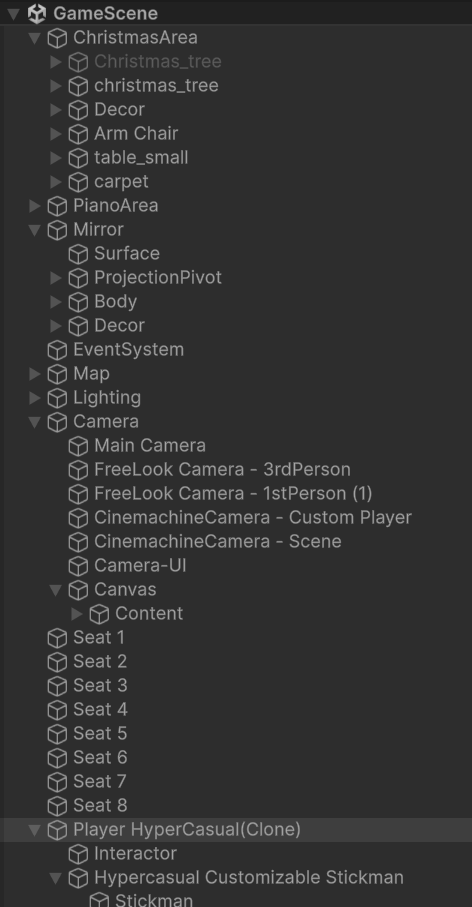
\includegraphics[width=3cm]{5.Thiết kế/images/game-object.png}
        \caption{Cấu trúc mẫu của các GameObject trong Scene (GameScene)}
        \label{fig:game-object}
    \end{figure}
    \newpage
    \item \textbf{Component}:
    \begin{enumerate}[-]
        \item Là nơi định nghĩa các hành vi và dữ liệu của GameObject. Ví dụ như Component Transform là một component bắt buộc có của mọi GameObject, nó giúp biểu diễn vị trí (tọa độ, hướng) và scale của đối tượng.
        \item Gồm các Component được viết sẵn của Unity và các script do lập trình tự viết. 
        \item Tính tái sử dụng cao, dễ mở rộng.
    \end{enumerate}
    \begin{figure}[!h]
        \centering
        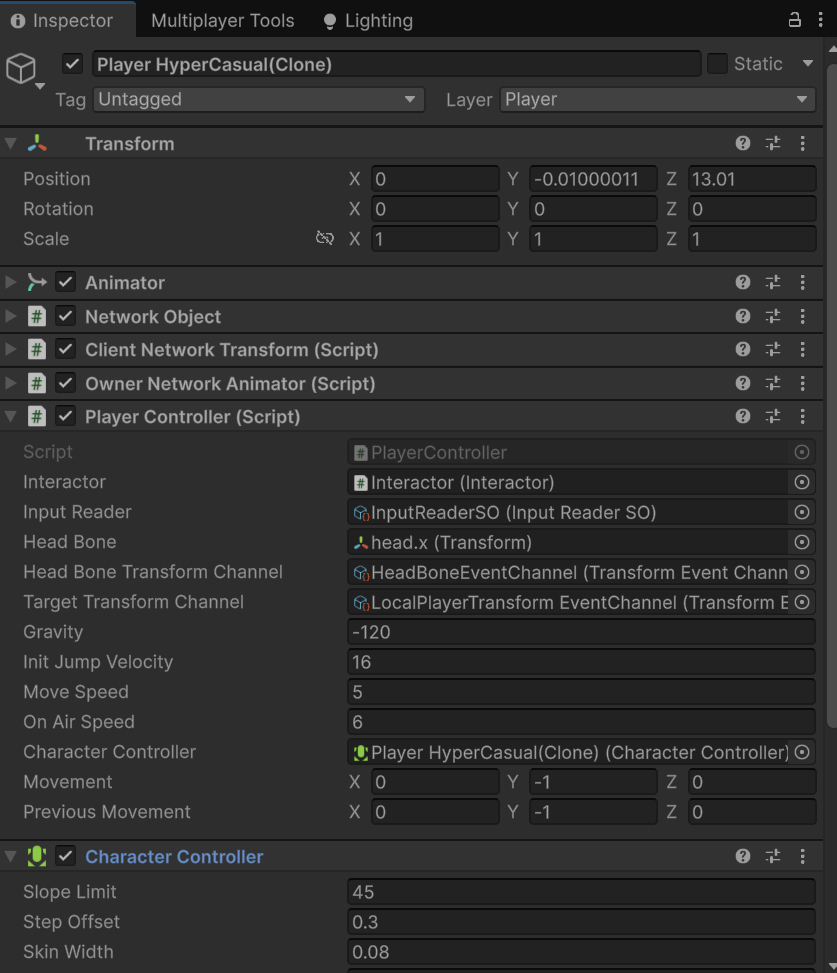
\includegraphics[width=8cm]{5.Thiết kế/images/component.png}
        \caption{Cấu trúc mẫu của các Component trong GameObject (Player)}
        \label{fig:component}
    \end{figure}
    \item \textbf{MonoBehaviour}:
    \begin{enumerate}[-]
        \item Là một class nền tảng của Unity Engine, cung cấp các callback trong lifecycle của Unity:
        \begin{enumerate}[+]
            \item Awake(): khởi tạo dữ liệu của class, chạy khi object được load vào Scene.
            \item Start(): chạy duy nhất 1 lần ngay trước frame đầu tiên sau khi object được kích hoạt.
            \item Update(): chạy mỗi frame khi được kích hoạt.
            \item FixUpdate(): tương tự Update nhưng FPS được giữ cố định, thường dùng cho các logic vật lý.
            \item LateUpdate(): chạy ngay sau Update chạy xong.
            \item OnEnable()/OnDisable(): chạy khi đối tượng được bật/tắt.
            \item OnDestroy(): Chạy khi object bị xóa khỏi Scene, dùng để dọn dẹp tài nguyên.
        \end{enumerate}
        \item Hỗ trợ liên kết dữ liệu giữa các component với hệ thống của Unity, hỗ trợ lập trình event-driven.
    \end{enumerate}
    \newpage
    \item \textbf{ScriptableObject}:
    \begin{enumerate}[-]
        \item Là một asset chứa dữ liệu, độc lập với scene và lifetime của Unity.
        \item Thường dùng lưu trữ dữ liệu tĩnh, có thể tái sử dụng cho nhiều đối tượng như Stats nhân vật, Skill data, Game Config...
        \item Phù hợp cho mô hình Data-Oriented.
    \end{enumerate}
    \begin{figure}[!h]
        \centering
        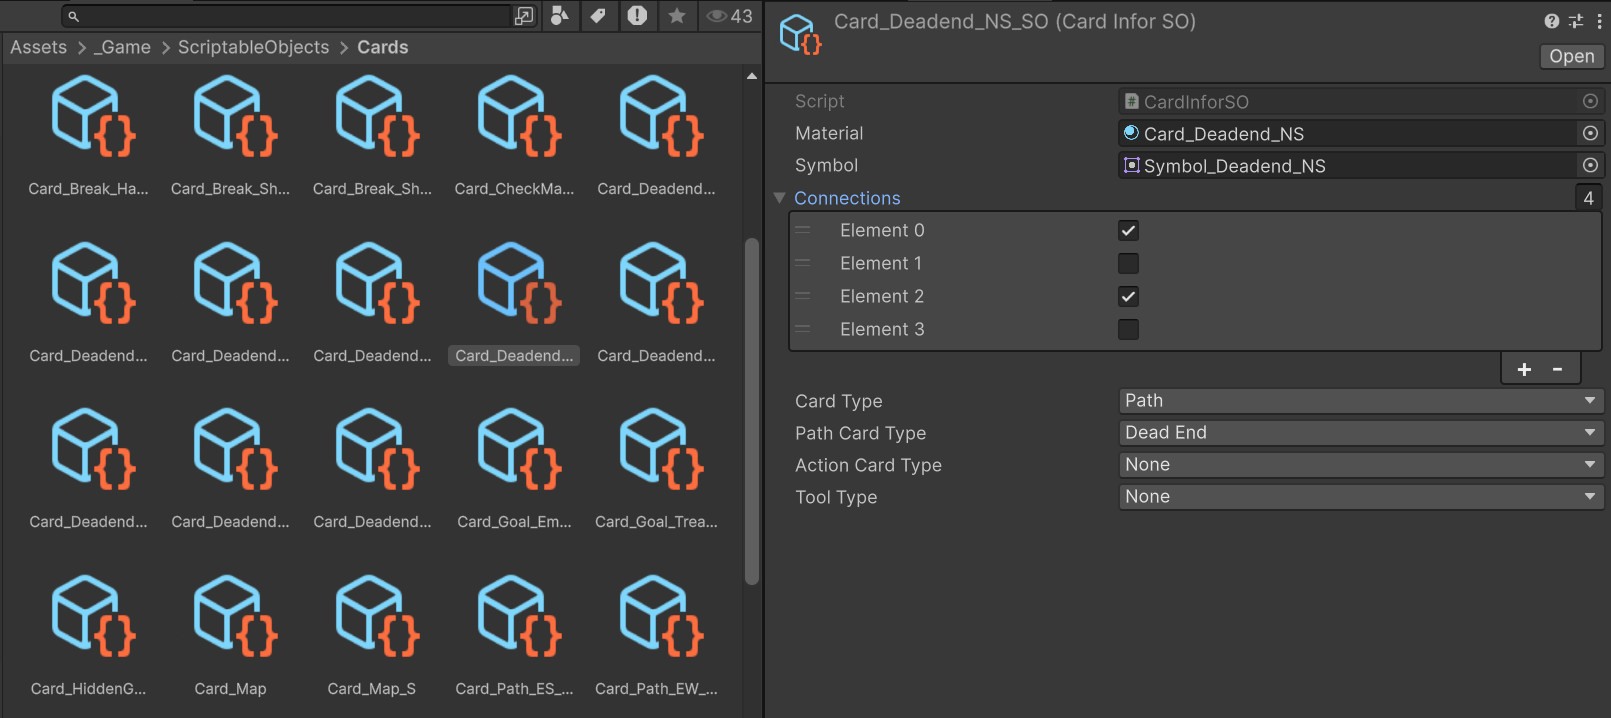
\includegraphics[width=10cm]{5.Thiết kế/images/scriptable-object.png}
        \caption{Các scriptable object sử dụng để lưu dữ liệu Card trong game}
        \label{fig:scriptable-object}
    \end{figure}
    \newpage
    \item \textbf{Prefab}:
    \begin{enumerate}[-]
        \item Là một asset lưu trữ toàn bộ thông tin của một GameObject.
        \item Dùng để tái sử dụng các đối tượng trong game như nhân vật, card ...
        \item Có cơ chế Prefab Variant giúp tạo các Prefab con kế thừa Prefab gốc (Prefab cha thay đổi thì Prefab con cũng thay đổi theo).
    \end{enumerate}
    \begin{figure}[!h]
        \centering
        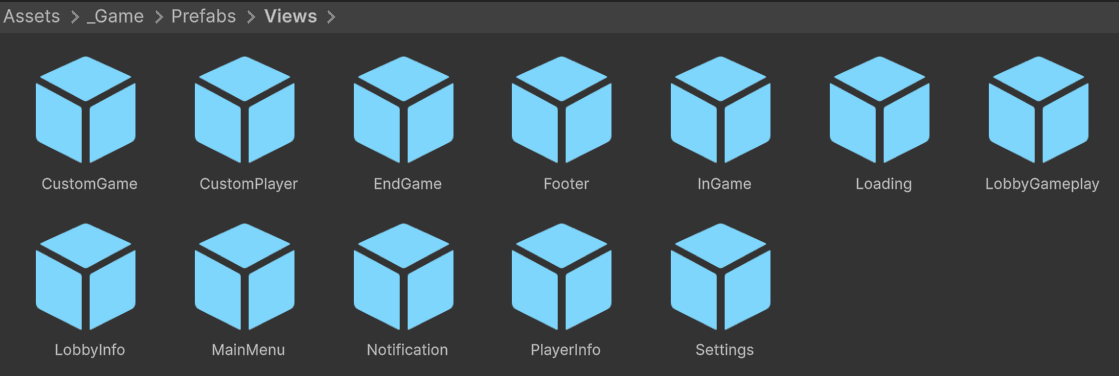
\includegraphics[width=10cm]{5.Thiết kế/images/prefab.png}
        \caption{Các prefab lưu trữ GameObject của UI các screen trong game}
        \label{fig:prefab}
    \end{figure}
    \item \textbf{Scene}:
    \begin{enumerate}[-]
        \item Là không gian chứa tất cả các GameObject.
        \item Thường được chia ra theo module để dễ quản lý: Boot Scene, Gameplay...
        \item Có thể mở nhiều scene cùng lúc (thường dùng cho tách riêng scene UI và scene gameplay).
    \end{enumerate}
   
\end{enumerate}
\subsubsection{Kiến trúc NGO}
NGO là công cụ hỗ trợ xây dụng game multiplayer dựa theo mô hình GameObject do Unity phát triển. NGO có mục tiêu chính là đơn giản hóa các đồng bộ trạng thái, xử lý RPC (remote procedure call), quản lý các kết nối người dùng trong mạng, đồng thời hỗ trợ các kiến trúc mạng khác nhau như client-host và client-server authoritative,

Trong NGO, vòng đời mạng tổng quan như sau:
\begin{enumerate}[+]
    \item Khởi tạo \textbf{NetworkManager}.
    \item Chọn chế độ chạy: Host/Client/Server.
    \item Server khởi tạo danh sách các kết nối.
    \item Server tạo các NetworkObject và thông báo tới Client.
    \item Client tạo bản sao và đồng bộ các trạng thái.
    \item Vòng lặp cập nhật (network tick), xử lý RPC.
    \item Dọn dẹp khi kết thúc: hủy các NetworkObject và hủy các kết nối mạng.
\end{enumerate}

Sau đây, nhóm sẽ giới thiệu các thành phần chính được sử dụng trong một dự án dùng NGO:
\begin{enumerate}[$\bullet$]
    \item \textbf{NetworkManager}:
    \begin{enumerate}[-]
        \item Là thành phần (Component) điều khiển chính của hệ thống mạng, quản lý đồng thời nhiều chức năng:
        \begin{enumerate}[+]
            \item Khởi tạo server, host hoặc client.
            \item Điều khiển tầng vận chuyển (Unity Transport/Custom Transport)
            \item Kiểm soát cập nhật mạng (tick mạng).
            \item Quản lý lifecycle của các NetworkObject trong mạng (tạo/hủy)
            \item Lưu trữ trạng thái, thông tin của các đối tượng kết nối trong mạng (client, server).
        \end{enumerate}
        \item Giao thức mặc định sử dụng là Unity Transport (UTP) hỗ trợ UDP tin cậy, QoS, kết hợp với Relay thông qua Unity Service, 
    \end{enumerate}   
    \item \textbf{NetworkObject}:
    \begin{enumerate}[-]
        \item Là Component bắt buộc cho bất ký GameObject nào muốn tồn tại trong mạng multiplayer, có vai trò quan trọng:
        \begin{enumerate}[+]
            \item Cung cấp mã định danh duy nhất (NetworkInstanceId) giữa tất cả các client.
            \item Quy định ai là chủ sở hữu (owner) của object.
        \end{enumerate}
        \item Chịu sử quản lý của NetworkManager khi tạo/hủy. Các thao tác server thực hiện để tạo (spawn) một NetworkGameobject:
        \begin{enumerate}[+]
            \item Server tạo instance trong scene.
            \item Object sẽ được cấp mã định danh.
            \item Server gửi thông báo đến tất cả các client.
            \item Client tạo bản sao tương ứng với NetworkObject được tạo trên server,
        \end{enumerate}
    \end{enumerate}
    \item \textbf{NetworkBehaviour}:
    \begin{enumerate}[-]
        \item Là một Component kế thừa từ MonoBehaviour và có thêm thêm các tính năng về mạng:
        \begin{enumerate}[+]
            \item Hỗ trợ RPC.
            \item Có thể sở hữu được NetworkVariable.
            \item Hỗ trợ các callback mạng như: OnNetworkSpawn(), OnNetworkDespawn(),...
        \end{enumerate}
        \item Được sử dụng đồng thời với MonoBehaviour để tách riêng logic runtime và các logic mạng:
        \begin{enumerate}[+]
            \item MonoBehaviour: xử lý input, animation, các UI local, audio...
            \item NetworkBehaviour: Xử lý đồng bộ, RPC, kiểm tra quyền,...
        \end{enumerate}
    \end{enumerate}
    \item \textbf{RPC (Remote Procedure Call)}:

    Là cơ chế gửi lời gọi hàm giữa client và server. Trong NGO cung cấp 2 loại RPC chính là ServerRpc và ClientRpc.
    \begin{enumerate}[-]
        \item \textbf{ServerRpc:}

        Gửi từ Client đến Server
        \begin{enumerate}[+]
            \item Đặc điểm: Chỉ chạy trên server, có thể được gửi từ owner hoặc non-owner, có hỗ trợ đảm bảo thứ tự và tin cậy.
            \item Ứng dụng: client gửi input cho server, gửi yêu cầu spawn object cho server (ví dụ như bán đạn), thông báo hành động (ví dụ như chọn bài).
        \end{enumerate}
        \item \textbf{ClientRpc:}

        Gửi từ Server đến Client
        \begin{enumerate}[+]
            \item Đặc điểm: Gửi đến mọi client hoặc một client cụ thể, thường dùng cho các sự kiện tức thời.
            \item Ứng dụng: Thông báo hiệu ứng (ví dụ như nổ, va chạm), cập nhật trạng thái (ví dụ như bắt đầu game).
        \end{enumerate}
    \end{enumerate}
    \item \textbf{NetworkVariable}:
    \begin{enumerate}[-]
        \item Là cơ chế giúp tối ưu quá trình đồng bộ dữ liệu game, tự động cập nhật trạng thái thay vì phải gửi RPC thủ công (giảm tải RPC).
        \item Hỗ trợ phân quyền đọc/ghi rõ ràng.
        \item Hỗ trợ callback khi giá trị thay đổi.
        \item Ứng dụng phổ biến trong đồng bộ thời gian (cooldown/countdown), điểm, máu...
    \end{enumerate}
    \item \textbf{NetworkList}:
    \begin{enumerate}[-]
        \item Là một dạng NetworkVariable chứa danh sách.
        \item Tự động đồng bộ các thay đổi trên danh sách (thêm, xóa, sửa) mà không cần gửi toàn bộ danh sách.
        \item Ứng dụng phổ biến với danh sách người chơi, kho đồ (inventory), bảng điểm,...
    \end{enumerate}
    \item \textbf{NetworkTransform}:
    \begin{enumerate}[-]
        \item Là Component chuyên dùng để tự động đồng bộ transform (vị trí, góc xoay, scale) của NetworkObject.
        \item Hỗ trợ tùy chỉnh thông số muốn đồng bộ để tối ưu tải.
        \item Hỗ trợ cơ chế interpolation giúp chuyển động mượt hơn.
    \end{enumerate}
\end{enumerate}
